\section{Parent selection functions}
Tournament selection reigned surpreme (fig \ref{fig:tournament}, epsilon=0.2, tournament size=8), averaging 12.55 generations (2.13 std) before finishing. This is a noticeable improvement from fitness proportionate (fig \ref{fig:fp}, 52 generations average, 12.61 std.

Sigma scaling (figure \ref{fig:sigma}) averaged 18.375 generations (4.37 std), placing itself firmly in the middle. Uniform selection with generational mixing (120 children, 80 adults) fared well (figure \ref{fig:uniform} 16.3 avg, 1.83 std) but this is due to the selection pressure of generational mixing, without which this selection mechanism devolves to random search.

One can see how the parent selection functions extending higher selection pressure fare much better in the simple One-Max problem. This especially due to the infrequency of local maxima, encouraging the greedy choice in most situations.

All averages were taken over a set of 100 runs.


\begin{figure}[H]
        \centering
        \begin{subfigure}[b]{0.5\textwidth}
                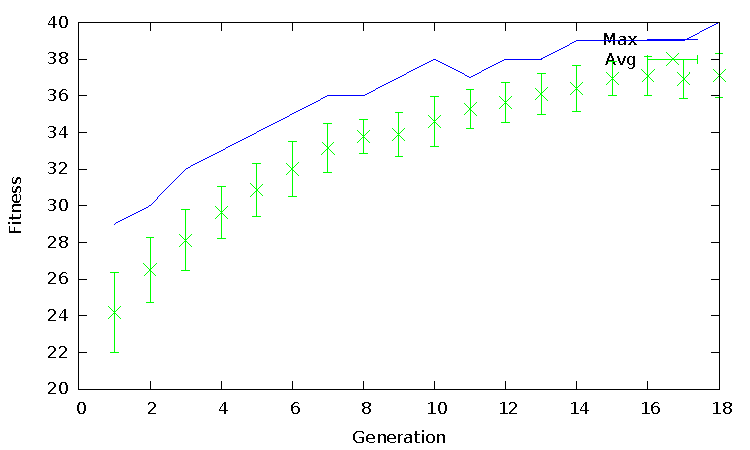
\includegraphics[width=\textwidth]{../results/other-functions/sigma-80-1.pdf}
                \caption{Sigma-scaling. Using a linearly rewarding fitness function}
                \label{fig:sigma}
        \end{subfigure}%
        \begin{subfigure}[b]{0.5\textwidth}
                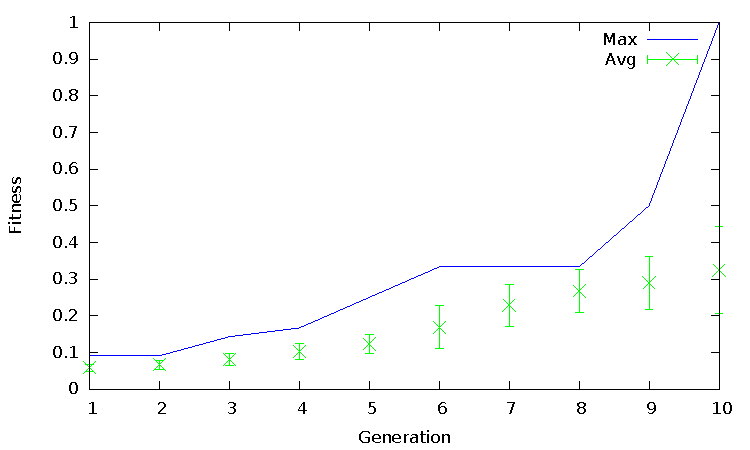
\includegraphics[width=\textwidth]{../results/other-functions/tournament-8-02.pdf}
                \caption{Tournament selection (epsilon=0.2, tournament size=8}
                \label{fig:tournament}
        \end{subfigure}
        \begin{subfigure}[b]{0.5\textwidth}
                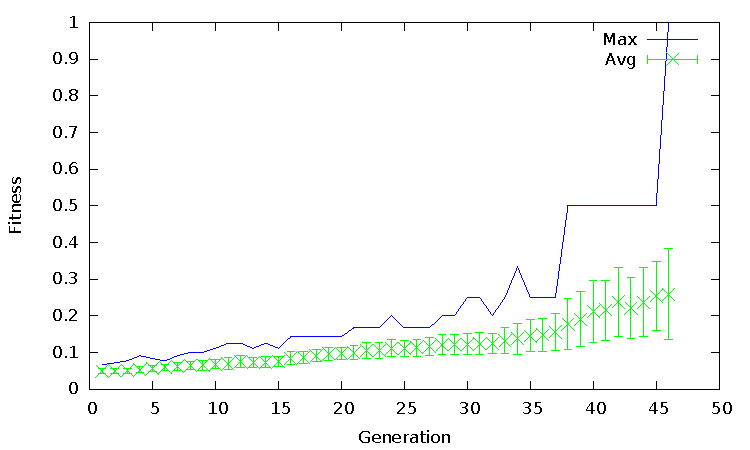
\includegraphics[width=\textwidth]{../results/omx-fgr-fp/omx-80-1-001.pdf}
                \caption{Fitness proportionate}
                \label{fig:fp}
        \end{subfigure}%
        \begin{subfigure}[b]{0.5\textwidth}
                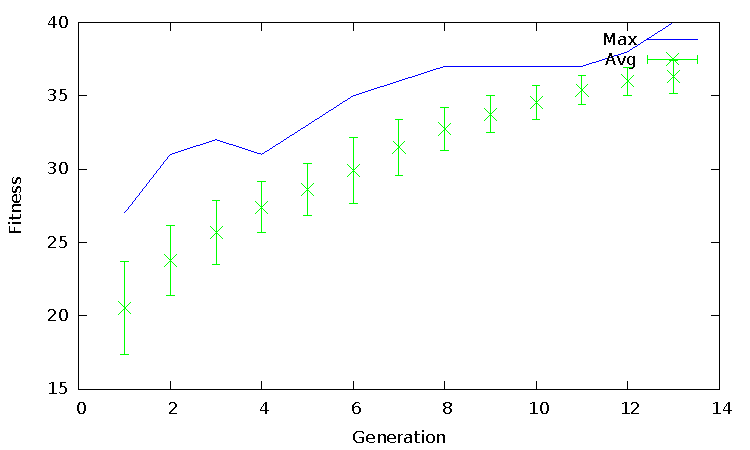
\includegraphics[width=\textwidth]{../results/other-functions/uniform-80-001.pdf}
                \caption{Uniform selection with gen. mixing}
                \label{fig:uniform}
        \end{subfigure}
        \caption{Different adult selection algorithms, all ran with mutation=0.01, crossover=1, and population size=80}
        \label{fig:fgp-fp-fitness-graphs}
\end{figure}